\documentclass[crop=false]{standalone}

\begin{document}
	\section{Expected Result}
	 
	 The experimental setup of this study assumes that the drone moves forward at a fixed altitude and speed. Three parameters are given: 1) the initial coordinate position of the drone, 2) the target endpoint, and 3) the positions of randomly generated obstacles, which serve as the second input parameter. Upon receiving these input parameters, the drone is expected to adjust its forward direction after takeoff. Since the drone moves at a fixed speed, it only needs to continuously calculate the distance to obstacles, maintain a safe distance from them, adjust its direction to avoid obstacles, and simultaneously move toward the endpoint. In summary, we expect that by using the DWA method, the drone will be able to navigate around obstacles and move steadily toward its destination, as shown in Figure 2:  
	
	\begin{figure}[htbp]	
		\centering
		\begin{minipage}{0.49\linewidth}
			\centering
			\fbox{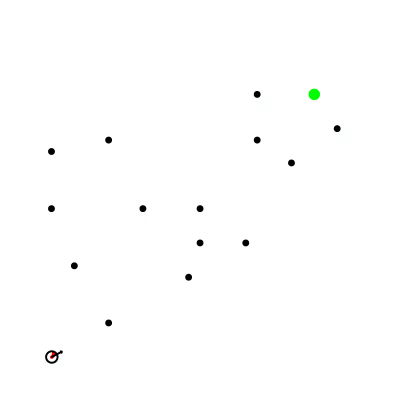
\includegraphics[width=0.8\linewidth]{dwa_frame_0.png}}
			\caption{Initial point}
			\label{Initial robot point}%文中引用该图片代号
		\end{minipage}
		\begin{minipage}{0.49\linewidth}
			\centering
			\fbox{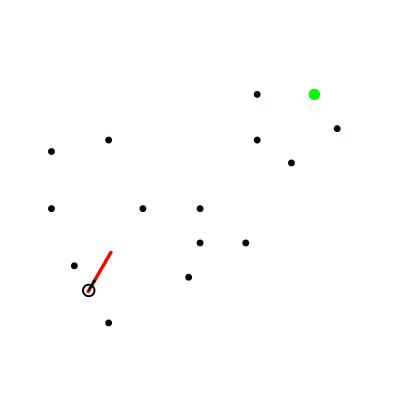
\includegraphics[width=0.8\linewidth]{dwa_frame_1.png}}
			\caption{Robot is moving}
			\label{Moving robot}%文中引用该图片代号
		\end{minipage}
		%\qquad
		%让图片换行,
		
		\begin{minipage}{0.49\linewidth}
			\centering
			\fbox{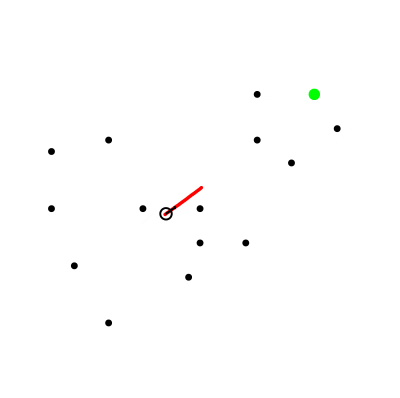
\includegraphics[width=0.8\linewidth]{dwa_frame_2.png}}
			\caption{Robot avoid obstacles}
			\label{Robot avoid obstacles}%文中引用该图片代号
		\end{minipage}
		\begin{minipage}{0.49\linewidth}
			\centering
			\fbox{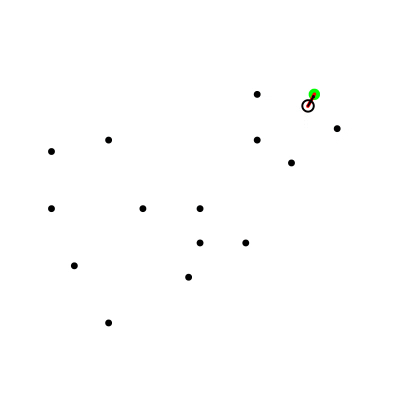
\includegraphics[width=0.8\linewidth]{dwa_frame_3.png}}
			\caption{Robot is arrived target point}
			\label{Robot is arrived target point}%文中引用该图片代号
		\end{minipage}
		
	\end{figure}
\end{document}

